\documentclass[11pt, openany, a4paper]{article}
\usepackage{etex}
\usepackage{fullpage}
\usepackage{pstricks,pstricks-add,pst-math,pst-xkey}
\usepackage[frenchb]{babel}
%\usepackage{slashbox}
\usepackage{graphicx}
\usepackage{amsmath,amssymb,amstext,amsthm}
\usepackage{mathtools}
%\usepackage{comment}
\usepackage[utf8]{inputenc}
\usepackage[OT1]{fontenc}
\usepackage{pgf,tikz}
\usepackage{pgfplots}
\usepackage{floatpag}
\usepgfmodule{shapes}
\usetikzlibrary{arrows,patterns}
\usepackage[ps]{skak}
\usepackage{chessboard}
\usepackage{floatflt}
\usepackage{import}
\newcounter{moncompteur}
\newtheorem{q}[moncompteur]{ \textbf{Question}}{}
\newtheorem{prop}[moncompteur]{ \textbf{Proposition}}{}
\newtheorem{df}[moncompteur]{ \textbf{Définition}}{}
\newtheorem*{df*}{ \textbf{Définition}}{}
\newtheorem{rem}[moncompteur]{ \textbf{Remarque}}{}
\newtheorem{theo}[moncompteur]{ \textbf{Théorème}}{}
\newtheorem{conj}[moncompteur]{ \textbf{Conjecture}}{}
\newtheorem{cor}[moncompteur]{ \textbf{Corollaire}}{}
\newtheorem{lm}[moncompteur]{ \textbf{Lemme}}{}
%\newtheorem{nota}[moncompteur]{ \textbf{Notation}}{}
%\newtheorem{conv}[moncompteur]{ \textbf{Convention}}{}
\newtheorem{exa}[moncompteur]{ \textbf{Exemple}}{}
\newtheorem{ex}[moncompteur]{ \textbf{Exercice}}{}
%\newtheorem{app}[moncompteur]{ \textbf{Application}}{}
%\newtheorem{prog}[moncompteur]{ \textbf{Algorithme}}{}
%\newtheorem{hyp}[moncompteur]{ \textbf{Hypothèse}}{}
\newenvironment{dem}{\noindent\textbf{Preuve}\\}{\flushright$\blacksquare$\\}
\newcommand{\cg }{[\kern-0.15em [}
\newcommand{\cd}{]\kern-0.15em]}
\newcommand{\R}{\mathbb{R}}
\newcommand{\K}{\mathbb{K}}
\newcommand{\N}{\mathbb{N}}
\newcommand{\Z}{\mathbb{Z}}
\newcommand{\C}{\mathbb{C}}
\newcommand{\U}{\mathbb{U}}
\newcommand{\Q}{\mathbb{Q}}
\newcommand{\B}{\mathbb{B}}
\newcommand{\card}{\mathrm{card}}
\newcommand{\norm}[1]{\left\lVert#1\right\rVert}
\pgfplotsset{compat=newest}
\newcommand{\La}{\mathcal{L}}
\newcommand{\Ne}{\mathcal{N}}
\newcommand{\D}{\mathcal{D}}
\newcommand{\Ss}{\textsc{safestay}}
\newcommand{\Sg}{\textsc{safego}}
\newcommand{\M}{\textsc{move}}
\newcommand{\E}{\mathcal{E}}
\newcommand{\V}{\mathcal V}
\setlength{\parindent}{0pt}
\newcommand{\myrightleftarrows}[1]{\mathrel{\substack{\xrightarrow{#1} \\[-.6ex] \xleftarrow{#1}}}}
\newcommand{\longrightleftarrows}{\myrightleftarrows{\rule{1cm}{0cm}}}

\newcommand\tikzmark[1]{%
  \tikz[overlay,remember picture,baseline] 
  \node[anchor=base](#1){};}

\newcommand\MyLine[3][]{%
  \begin{tikzpicture}[overlay,remember picture]
    \draw[#1] (#2.north west) -- (#3.south east);
  \end{tikzpicture}}


\graphicspath{{.}}
\newcommand{\e}[1]{$\times 10^{#1}$}

\begin{document}
\floatpagestyle{plain}
\renewcommand{\labelitemi}{$\bullet$}

\title{\vspace{-3em}Multiplication binaire et factorisation}
\date{Juin-Juillet 2014}
\author{Raphaël Rieu-Helft}

\maketitle

\part*{Introduction}

Ce stage...

%%%%%%%%%%%%%%%%%%%%%%%%%%%%%%%%%%%%%%%%%%%%%%%%%%%%%%%%%%%%%%%%%%%%%%%%%%%%%%%%
% N-REINES
%%%%%%%%%%%%%%%%%%%%%%%%%%%%%%%%%%%%%%%%%%%%%%%%%%%%%%%%%%%%%%%%%%%%%%%%%%%%%%%%
\part{Le problème des $n$ reines}
\label{part:nreines}

%\section{Introduction}
\section{Position du problème}
\label{sec:intronreines}

%\ANNOT{...\cite{BahiC06}, \cite{ChevFat08,Fat13}... citations liées aux n reines  ...
%}


On se place sur un échiquier de  taille $n \times n$, sur lequel~$n$ reines sont
disposées. On dit qu'une reine est  \emph{menacée} si elle se trouve sur la même
ligne,  colonne ou diagonale  qu'une autre  reine. On  cherche à  placer les~$n$
reines de sorte qu'aucune reine ne soit menacée.
On va chercher,  en partant d'une situation initiale  quelconque, à déplacer les
reines  de sorte à  atteindre une  position dans  laquelle aucune  d'elles n'est
menacée. Pendant ces déplacements, on va  permettre à chaque case de contenir un
nombre  quelconque de  reines simultanément,  et  aussi d'être  marquée par  des
signaux  provenant  d'un nombre  quelconque  de  directions,  qui traduisent  la
présence d'une reine dans la direction d'où ils proviennent. %
% Notons  donc $\B$  l'ensemble $\{vrai,  faux\}$  des booléens.   On associe  à
% chaque case  de coordonnées  $(i,j)$ un état  $x_{i,j} \in  \B^8\times\N$. Les
% huit booléens  correspondent à  la présence ou  à l'absence, en  provenance de
% chacune des  huit directions, d'un  signal traduisant la présence  d'une reine
% dans  cette direction, et  l'entier (compris  entre~$0$ et~$n$)  correspond au
% nombre de reines présentes sur la case.
% On dit  qu'une case est \emph{sûre}  si elle ne  contient pas de signal  ni de
% reine (état $(faux,  faux, ..., faux, 0)$)  et on entend par là  que c'est une
% bonne case de  destination pour une reine. Dans le cas  contraire, la case est
% dite \emph{dangereuse}.


\begin{floatingfigure}[r]{.5\textwidth}
\centering
\newgame
\fenboard{7q/6q1/5q2/4q3/3q4/2q5/1q6/q7 b - - 0 1}
\notationoff
\showboard
\caption{Les reines sont toutes menacées, mais aucun déplacement d'une case ne conduit à une case sûre.}
\label{fig:blocage}
\end{floatingfigure} 
On cherche une procédure de mise à jour locale telle qu'à chaque pas
de temps, les états de certaines cases sont modifiés à partir d'informations sur
les  cases voisines  :  création  et transmission  de  signaux, déplace\-ments  de
reines... L'objectif est que  les signaux  tradui\-sent au  mieux la  présence de reines  dans la  direction d'où  ils vien\-nent,  et que  les reines
menacées  se déplacent  au cours  du  temps pour  chercher des  cases sûres.  On
cherche également à  ce que les reines ne bougent plus  une fois qu'une solution
est atteinte. On s'astreint à ne déplacer les reines  que d'au plus une case par pas de temps,
de sorte que la règle de mise  à jour puisse rester purement locale.

On voudrait ne déplacer les reines que sur des  cases sûres, mais c'est trop restrictif : il
existe des  positions qui ne  sont pas solution  du problème mais où  toutes les
reines  sont  entourées de  cases  menacées  (cf. Figure~\ref{fig:blocage}).  En
revanche, permettre  aux reines  de se déplacer  sur des cases  dangereuses sans
utiliser les informations locales dont elles disposent donne des mouvements trop
aléatoires  pour  qu'on  puisse  espérer  atteindre une  solution  en  un  temps
raisonnable.  On  fixe  donc   une  probabilité  $\varepsilon  \in  [0,1]$,  qui
correspond à la probabilité pour une  reine qui envisage un déplacement vers une
case dangereuse de  l'effectuer, alors qu'un déplacement vers  une case sûre est
systé\-ma\-tique.  En fixant  $\varepsilon$ assez  petit (de  l'ordre de  $0.01$ par
exemple), on privilégie les déplacements vers des cases sûres tout en se donnant
quand même la possibilité de sortir de situations bloquées.


%\section*{La procédure de mise à jour}
\section{Formalisation}

\subsection{Représentation du système}

\noindent
On représente l'échiquier par l'ensemble $\La = \cg 0, n-1\cd^2$. On pose
$\mathcal{P} = \{0,1\}$ et \linebreak $\D = \{NW,N,NE,W,E,SW,S,SE\}$ l'ensemble des huit directions. L'état d'une cellule étant déterminé par le nombre de reines présentes et la présence ou l'absence d'un signal en provenance de chaque direction, on note $\mathcal{Q} = {\mathcal{P}^8}\times\N$ l'ensemble des états. Une \emph{configuration} est un élément de $\E=\mathcal{Q}^\La$. Pour toute configuration~$x$, et toute cellule $c \in \La$, on note $x_c = (s_{x, c}, n_{x, c})$ l'état de la cellule~$c$ dans la configuration~$x$, où $n_{x,c}$ est le nombre de reines sur la cellule~$c$ dans la configuration~$x$, et $s_{x,c} = (s_{x,c,N}, s_{x,c,NE}, s_{x,c,E}, \ldots, s_{x,c,NW})$ code la présence ou l'absence de signaux venant de chaque direction : $s_{x,c,d}$ vaut~$1$ si dans la configuration~$x$, la cellule~$c$ contient un signal provenant de la direction~$d$, et~$0$ sinon.


Par souci de lisibilité, on omettra les indices~$x$ de configuration partout où on pourra le faire sans ambiguïté et on parlera de l'état $(s_c, n_c)$ d'une cellule~$c$.
%La fonction $s_{x, c}$ associe à chaque direction~$1$ si~$c$ contient un signal en provenance de cette direction et~$0$ sinon, et~$c$ contient $n_{x, c}$ reines.

On pose $\Ne \subset \La^2$ l'ensemble des paires de cellules adjacentes : $$(c, c') \in \Ne \iff \norm{(c-c')}_\infty = 1$$

À chaque pas de temps, on choisit au hasard une paire de cases adjacentes et on les met à jour l'une par rapport à l'autre.
On se donne donc $(u_t)_{t\in\N} \in \Ne^\N$ la suite des paires de cellules mises à jour : pour tout $t\in\N$, la paire de cellules mises à jour à l'étape~$t$ est $u_t$. Ce sont les valeurs d'une suite de variables aléatoires indépendantes à distribution uniforme sur $\Ne$. On définit de même $(x_t)_{t\in\N}$ la suite des configurations prises par le système au cours du temps. Initialement, aucun signal n'est présent et les~$n$ reines sont réparties aléatoirement sur l'échiquier, selon une loi uniforme (de façon indépendante : notamment plusieurs reines peuvent se trouver initialement sur la même case). 
On cherche à définir une fonction de mise à jour globale $\mathcal{F} : {\E\times\Ne}\to\E$ qui à une configuration associe une configuration qui lui succède selon la procédure de la partie précédente : \mbox{$\mathcal{F}(x_t, u_t) = x_{t+1}$}.

%Initialement, aucun signal n'est présent.
% et les~$n$ reines sont réparties aléatoirement sur l'échiquier, selon une loi uniforme (de façon indépendante : notamment plusieurs reines peuvent se trouver initialement sur la même case). 
 
\subsection{Choix des cases à mettre à jour}

On souhaite choisir une paire de cases adjacentes à mettre à jour, avec la même probabilité de choisir chaque paire de cases. On observe qu'il y a $n(n-1)$ paires de cases voisines verticalement, $n(n-1)$ horizontalement et $(n-1)^2$ selon chaque diagonale, soit $(4n-2)(n-1)$ paires de cases adjacentes au total. On applique donc la procédure de sélection suivante : \begin{itemize}

\item{On choisit selon une loi uniforme $N \in \cg 0, (4n-2)(n-1) -1 \cd$, on en déduit $A \in \cg 0, 4n-3 \cd$ et $B \in \cg 0, n-2\cd$ le quotient et le reste de la division euclidienne de~$N$ par $(n-1)$.  }
\item{Si $A<n$, on prend les cases $(B,A)$ et $(B+1,A)$.}
\item{Si $A = n+i, 0\leq i<n$, on prend les cases $(i,B)$ et $(i,B+1)$.}
\item{Si $A = 2n+i,0 \leq i<n-1$, on prend $(i,B)$ et $(i+1, B+1)$.}
\item{Sinon, $A = 3n-1+i$ et $0 \leq i<n-1$, et on prend $(i, B+1)$ et $(i+1, B)$.}
%\item{On choisit selon une loi uniforme une direction (parmi N, NW, NE, W, E, SW, SE, S)}.

%\item{On choisit selon une loi uniforme une case possédant une case voisine dans cette direction (c'est-à-dire ne se trouvant pas sur le mauvais bord de l'échiquier).}

%\item{Les cases à mettre à jour sont la case tirée au sort et sa voisine dans la direction tirée au sort.}

\end{itemize}
La fonction qui à~$N$ associe une paire de cases adjacentes étant bijective, on a bien la même probabilité de choisir chaque paire de cases. 


\subsection{Mise à jour : les déplacements}

\definecolor{ffqqqq}{rgb}{1,0,0}
\definecolor{xdxdff}{rgb}{0.49,0.49,1}
\definecolor{zzttqq}{rgb}{0.6,0.2,0}
\definecolor{uququq}{rgb}{0.25,0.25,0.25}
\definecolor{qqqqff}{rgb}{0,0,1}

\begin{figure}[t]
  \centering
  \resizebox{.5\textwidth}{!}{
    \begin{tikzpicture}[line cap=round,line join=round,>=triangle 45,x=1.0cm,y=1.0cm]
      \clip(-8.56,-0.74) rectangle (4.7-2.5,2.48);
      % \fill[color=zzttqq,fill=zzttqq,fill opacity=0.1] (0,2) -- (0,0) -- (2,0) -- (2,2) -- cycle;
      % \fill[color=zzttqq,fill=zzttqq,fill opacity=0.1] (2,2) -- (2,0) -- (4,0) -- (4,2) -- cycle;
      % \fill[color=zzttqq,fill=zzttqq,fill opacity=0.1] (-7.7,2) -- (-7.7,0) -- (-5.7,0) -- (-5.7,2) -- cycle;
      % \fill[color=zzttqq,fill=zzttqq,fill opacity=0.1] (-5.7,2) -- (-5.7,0) -- (-3.7,0) -- (-3.7,2) -- cycle;
      \draw [color=zzttqq] (0-2.5,2)-- (0-2.5,0);
      \draw [color=zzttqq] (0-2.5,0)-- (2-2.5,0);
      \draw [color=zzttqq] (2-2.5,0)-- (2-2.5,2);
      \draw [color=zzttqq] (2-2.5,2)-- (0-2.5,2);
      \draw [color=zzttqq] (2-2.5,2)-- (2-2.5,0);
      \draw [color=zzttqq] (2-2.5,0)-- (4-2.5,0);
      \draw [color=zzttqq] (4-2.5,0)-- (4-2.5,2);
      \draw [color=zzttqq] (4-2.5,2)-- (2-2.5,2);
      \draw [->] (2-2.5,1) -- (1.5-2.5,1);
      \draw (1.02-2.5,-0.14) node[anchor=north west] {\Large 1};
      \draw (2.94-2.5,-0.14) node[anchor=north west] {\Large 2};
      \draw [color=zzttqq] (-7.7,2)-- (-7.7,0);
      \draw [color=zzttqq] (-7.7,0)-- (-5.7,0);
      \draw [color=zzttqq] (-5.7,0)-- (-5.7,2);
      \draw [color=zzttqq] (-5.7,2)-- (-7.7,2);
      \draw [color=zzttqq] (-5.7,2)-- (-5.7,0);
      \draw [color=zzttqq] (-5.7,0)-- (-3.7,0);
      \draw [color=zzttqq] (-3.7,0)-- (-3.7,2);
      \draw [color=zzttqq] (-3.7,2)-- (-5.7,2);
%      \draw [->,dash pattern=on 1pt off 1pt,very thick] (-3.1,1) --      (-0.58-1.5,1);
      \draw (-3.1,1) node {\Huge$\Rightarrow$};
      \draw (-6.94,-0.22) node[anchor=north west] {\Large 1};
      \draw (-4.66,-0.2) node[anchor=north west] {\Large 2};
      \draw [->] (-6.7,2) -- (-6.7,1.5);
      \draw [->] (1-2.5,2) -- (1-2.5,1.5);
      \draw [fill=black,pattern=north east lines] (-6.74,0.96) circle (0.29cm);
      \draw [fill=black,pattern=north east lines] (3.04-2.5,1.02) circle (0.29cm);
    \end{tikzpicture}
  }
  % \includegraphics[scale=1.2]{schema2.png}
  \caption{La reine présente  en 1, menacée depuis le nord, se  déplace en 2 qui
    est une case sûre, puis les signaux sont mis à jour : il y a une reine en 2,
    donc un signal venant de l'est apparaît en 1.}
  \label{fig:deplacement}
%\ANNOT{Voir  comment  j'ai  réduit  la  figure  2  (agrandissement  des  textes, remplacement de la flèche par une flèche  math, et décalage en x pour tous les x $>$ à la pointe de la flèche initiale (un copier-coller de -2.5 suffit)}
\end{figure}


On se donne  deux cases adjacentes~$c$ et~$c'$ à mettre à  jour. On commence par
envisager des déplacements  de reine entre~$c$ et~$c'$. Le  principe général est
qu'une reine menacée  essaie de quitter sa case lorsqu'elle est  mise à jour. Ce
déplacement réussit  ou non en fonction de  l'état de l'autre case  mise à jour,
avec une part d'aléatoire. 
La procédure est la suivante :
\begin{itemize}
\item Si une reine est présente en case~$c$, alors que la case~$c$ contient un signal, elle essaie de se déplacer vers la case~$c'$. De même, si plusieurs reines sont présentes en~$c$, elles sont menacées et l'une d'entre elles tente de se déplacer vers la case~$c'$.
\item S'il n'y a pas de signal en~$c'$ sauf éventuellement un venant de~$c$ (qui est peut-être dû à la présence de la reine qui cherche à bouger), et qu'il n'y a pas d'autre reine en~$c'$, la case est considérée comme sûre et le déplacement a lieu (cf. Figure~\ref{fig:deplacement}). Sinon, la case est dangereuse, et le déplacement a lieu seulement avec une probabilité $\varepsilon$.
% Si le déplacement réussit, on retire une reine à la case~$c$ et on en ajoute une à la case $(i', j')$. 
\item Symétriquement, une reine de~$c'$ peut se déplacer vers~$c$ selon la même procédure. Les deux déplacements se font de manière simultanée afin que l'ordre des deux cases choisies pour la mise à jour n'ait pas d'importance.
\end{itemize}



Formalisons cette procédure à l'aide de quelques fonctions auxiliaires :  

 \begin{itemize}
  \item On pose $\Ss : {\La}\to\{0,1\}$ qui indique si une reine peut rester sur une case donnée : \[
 \Ss(c) =
  \begin{cases} 
      \hfill 1    \hfill & \text{ si $n_c\leq 1$ et $\forall d \in \D, s_c(d)=0$} \\
      \hfill 0 \hfill & \text{ sinon} \\
  \end{cases}
\]
 
  \item On pose $\Sg :  {\La\times\D}\to\{0,1\}$ qui indique si une reine peut se déplacer de façon sûre vers une certaine case en venant d'une certaine direction : \[
 \Sg(c, d_{\mathrm {from}}) =
  \begin{cases} 
      \hfill 1    \hfill & \text{ si $n_c=0$ et $\forall d \in \D\setminus\{d_{\mathrm{from}}\}, s_c(d)=0$} \\
      \hfill 0 \hfill & \text{ sinon} \\
  \end{cases}
\]
 En toute rigueur, $\Ss$ et $\Sg$ devraient prendre aussi la configuration en argument : on l'omet pour plus de lisibilité.

%\medskip
  \item On pose $\delta :\Ne\to\D$ telle que $\delta(c_{\mathrm{from}}, c_{\mathrm{to}})$ soit la direction de $c_{\mathrm{from}}$ vue de $c_{\mathrm{to}}$. Plus formellement : \[
 \delta(c_{\mathrm{from}}, c_{\mathrm{to}}) =
  \begin{cases} 
    \hfill N    \hfill & \text{ si $c_{\mathrm{to}}-c_{\mathrm{from}}=(0,1)$} \\
    \hfill NE \hfill & \text{ si  $c_{\mathrm{to}}-c_{\mathrm{from}}=(1,1)$} \\
    \hfill \cdots & \\
    \hfill W \hfill & \text{ si  $c_{\mathrm{to}}-c_{\mathrm{from}}= (-1,0)$}\\
    \hfill NW \hfill & \text { si  $c_{\mathrm{to}}-c_{\mathrm{from}}=(-1,1)$}\\
  \end{cases}
\] 
  \item On peut alors définir $\M :{\Ne}\to\{0,1\}$ qui traduit la procédure décrite ci-dessus : $\M(c_{\mathrm{from}}, c_{\mathrm{to}})$ vaut~$1$ si une reine se déplace de $c_{\mathrm{from}}$ à $c_{\mathrm{to}}$ et~$0$ sinon. Formellement : \[
    \M(c_{\mathrm{from}}, c_{\mathrm{to}}) = 
    \begin{cases}
      \hfill 0 \hfill & \text{ si $\Ss(c_{\mathrm{from}})=1$} \\
      \hfill 1 \hfill & \text{ si : }{ \begin{cases} \Ss(c_{\mathrm{from}})=0 \\\text{et $n_{c_{\mathrm{from}}}\geq 1$} \\ \text{et } \Sg(c_{\mathrm{to}}, \delta(c_{\mathrm{from}}, c_{\mathrm{to}}))=1\\ \end{cases}}\\

      \hfill \mathcal{B}(\varepsilon)\hfill  & \text{ sinon} \\
    \end{cases}
\]
où $\mathcal{B}(\varepsilon)$ est une variable aléatoire valant~$1$ avec une probabilité $\varepsilon$ et~$0$ avec une probabilité $1-\varepsilon$. Comme précédemment, on omet de passer la configuration en argument à $\M$ tant qu'il n'y a pas d'ambiguïté.



\end{itemize}


On peut maintenant écrire $\mathcal{F}_{\mathrm{move}} : \E\times\Ne\to\E$ qui modifie la configuration par d'éventuels déplacements de reine entre les cases mises à jour :  \[
\mathcal{F}_{\mathrm{move}}(x,(c_1, c_2)) = 
\begin{cases}
  \hfill x_{c_1\to c_2} \hfill & \text{ si $\M(c_1, c_2) = 1$ et $\M(c_2, c_1) = 0$} \\
  \hfill x_{c_2 \to c_1} \hfill & \text{ si $\M(c_1, c_2) = 0$ et $\M(c_2, c_1) = 1$} \\
  \hfill x \hfill & \text{ sinon} \\
  \end{cases}
\]
où $x_{a \to b}$ désigne la configuration obtenue à partir de~$x$ en ôtant~$1$ à $n_{a}$ et en ajoutant~$1$ à $n_{b}$. 

\subsection{Mise à jour : les signaux}  

Après avoir effectué d'éventuels déplacements de reine, on met à jour les signaux de~$c$ et~$c'$. 

 \begin{itemize} 

\item{% Le signal en~$c'$ provenant de la direction de~$c$ est modifié de la façon suivante : il devient vrai 
Un signal en~$c'$ provenant de la direction de~$c$ apparaît ou reste présent s'il y a une reine en~$c$ (cf. Figure~\ref{fig:deplacement}), ou s'il y a un signal en~$c$ dans la même direction (intuitivement, il y a une reine plus loin dans la direction de~$c$) (cf. Figure~\ref{fig:transmission}). Sinon, rien n'indique plus la présence d'une reine dans cette direction : le signal disparaît s'il était présent (cf. Figure~\ref{fig:disparition}). }

\item{ Symétriquement, le signal en~$c$ provenant de~$c'$ est mis à jour de la même façon.}

\item{ Les autres signaux ne sont pas modifiés. }
  
%Le booléen de $x_{i,j}$ correspondant à la direction $d_{2\rightarrow 1}$ devient vrai s'il y a au moins une reine sur la case~$c'$ ou si le booléen de $x_{i',j'}$ correspondant à  $d_{2\rightarrow 1}$  est vrai (intuitivement, il y a alors une reine plus loin dans cette direction), et devient faux sinon.

% Symétriquement, le booléen de $x_{i', j'}$ correspondant à $d_{1\rightarrow 2}$ devient vrai s'il y a une reine en~$c$ ou si le booléen de $x_{i,j}$ correspondant à $d_{1\rightarrow 2}$ est vrai, et devient faux dans le cas contraire.}

\end{itemize}

\begin{figure}[hbt]
  \centering
  \begin{minipage}{.45\textwidth}
    \centering
    \resizebox{\columnwidth}{!}{
      \begin{tikzpicture}[line cap=round,line join=round,>=triangle 45,x=1.0cm,y=1.0cm]
        \clip(-8.56,-0.74) rectangle (4.7-2.5,2.48);
        % \fill[color=zzttqq,fill=zzttqq,fill opacity=0.1] (0,2) -- (0,0) -- (2,0)
        % -- (2,2) -- cycle;\fill[color=zzttqq,fill=zzttqq,fill opacity=0.1] (2,2)
        % -- (2,0) -- (4,0) -- (4,2) -- cycle; \fill[color=zzttqq,fill=zzttqq,fill
        % opacity=0.1] (-7.7,2) -- (-7.7,0) -- (-5.7,0) -- (-5.7,2) -- cycle;
        % \fill[color=zzttqq,fill=zzttqq,fill opacity=0.1] (-5.7,2) -- (-5.7,0) --
        % (-3.7,0) -- (-3.7,2) -- cycle;
        \draw [color=zzttqq] (0-2.5,2)-- (0-2.5,0);
        \draw [color=zzttqq] (0-2.5,0)-- (2-2.5,0);
        \draw [color=zzttqq] (2-2.5,0)-- (2-2.5,2);
        \draw [color=zzttqq] (2-2.5,2)-- (0-2.5,2);
        \draw [color=zzttqq] (2-2.5,2)-- (2-2.5,0);
        \draw [color=zzttqq] (2-2.5,0)-- (4-2.5,0);
        \draw [color=zzttqq] (4-2.5,0)-- (4-2.5,2);
        \draw [color=zzttqq] (4-2.5,2)-- (2-2.5,2);
        \draw [->] (0-2.5,2) -- (0.5-2.5,1.48);
        \draw [->] (0-2.5,1) -- (0.5-2.5,1); 
        \draw [->] (2-2.5,1) -- (2.5-2.5,1);
        \draw (1.02-2.5,-0.14) node[anchor=north west] {\Large 1};
        \draw(2.94-2.5,-0.14) node[anchor=north west] {\Large 2};
        \draw [color=zzttqq] (-7.7,2)-- (-7.7,0); 
        \draw [color=zzttqq] (-7.7,0)-- (-5.7,0); 
        \draw [color=zzttqq](-5.7,0)-- (-5.7,2);
        \draw [color=zzttqq] (-5.7,2)-- (-7.7,2); 
        \draw [color=zzttqq] (-5.7,2)-- (-5.7,0); 
        \draw [color=zzttqq] (-5.7,0)--(-3.7,0); 
        \draw [color=zzttqq] (-3.7,0)-- (-3.7,2); 
        \draw [color=zzttqq] (-3.7,2)-- (-5.7,2);
        \draw [->] (-7.7,2) -- (-7.2,1.5);
        \draw [->] (-7.7,1)  -- (-7.2,1);
        % \draw [->,dash pattern=on 1pt off 1pt] (-3.1,0.98) --  (-0.58,1); 
        \draw (-3.1,1) node {\Huge$\Rightarrow$};
        \draw (-6.94,-0.22) node[anchor=north west] {\Large 1}; 
        \draw (-4.66,-0.2) node[anchor=north west] {\Large 2};
      \end{tikzpicture} 
    } 
    \caption {Le signal de la cellule 1 venant de l'ouest est transmis à la cellule 2.}
    \label{fig:transmission}
    \end{minipage}   
    \quad
    \begin{minipage}{.45\textwidth} 
      \centering
    \resizebox{\columnwidth}{!}{
      \begin{tikzpicture}[line cap=round,line join=round,>=triangle 45,x=1.0cm,y=1.0cm]
        \clip(-8.56,-0.74) rectangle (4.7-2.5,2.48);
        \draw [color=zzttqq] (0-2.5,2)-- (0-2.5,0);
        \draw [color=zzttqq] (0-2.5,0)-- (2-2.5,0);
        \draw [color=zzttqq] (2-2.5,0)-- (2-2.5,2);
        \draw [color=zzttqq] (2-2.5,2)-- (0-2.5,2);
        \draw [color=zzttqq] (2-2.5,2)-- (2-2.5,0);
        \draw [color=zzttqq] (2-2.5,0)-- (4-2.5,0);
        \draw [color=zzttqq] (4-2.5,0)-- (4-2.5,2);
        \draw [color=zzttqq] (4-2.5,2)-- (2-2.5,2);
        \draw (1.02-2.5,-0.14) node[anchor=north west] {\Large 1};
        \draw (2.94-2.5,-0.14) node[anchor=north west] {\Large 2};
        \draw [color=zzttqq] (-7.72,2)-- (-7.72,0);
        \draw [color=zzttqq] (-7.72,0)-- (-5.72,0);
        \draw [color=zzttqq] (-5.72,0)-- (-5.72,2);
        \draw [color=zzttqq] (-5.72,2)-- (-7.72,2);
        \draw [color=zzttqq] (-5.72,2)-- (-5.72,0);
        \draw [color=zzttqq] (-5.72,0)-- (-3.72,0);
        \draw [color=zzttqq] (-3.72,0)-- (-3.72,2);
        \draw [color=zzttqq] (-3.72,2)-- (-5.72,2);
        % \draw [->,dash pattern=on 1pt off 1pt] (-3.1,0.98) -- (-0.58,1);
        \draw (-3.1,1) node {\Huge$\Rightarrow$};
        \draw (-6.94,-0.22) node[anchor=north west] {\Large 1};
        \draw (-4.66,-0.2) node[anchor=north west] {\Large 2};
        \draw [->] (-6.72,0) -- (-6.72,0.5);
        \draw [->] (1,0) -- (1,0.5);
        \draw [->] (-5.72,1) -- (-6.22,1);
      \end{tikzpicture}
      }
      \caption{Le signal en 1 venant de l'est disparaît.}
      \label{fig:disparition}
    \end{minipage}
%  }
\end{figure}


\noindent 
Formellement, on pose, pour tout %$x\in\E$, $(c,c')\in\Ne$, 
$d\in\D$,  $s_{x, c, d}^{c'}$ le signal de la case~$c$ se rapportant à la direction~$d$, mis à jour par rapport à~$c'$ selon la règle :  \[
s_{x, c, d}^{c'} = 
\begin{cases}
  \hfill s_{x, c, d} \hfill & \text{ si $d \neq \delta(c', c)$} \\
  \hfill 1 \hfill & \text{ si $d = \delta(c', c)$ et $n_{x, c'}\geq 1$} \\
  \hfill s_{x, c', d} \hfill & \text{ sinon}\\
\end{cases}
\]

On va s'en servir pour définir une fonction $\mathcal{F}_{\mathrm{sign}} : \E\times\Ne\to\E$ de mise à jour des signaux :
\noindent
 $\mathcal{F}_{\mathrm{sign}} (x, (c_1, c_2)) = x'$ avec : \[
\begin{cases}
  \hfill x'_{c_1} = (s_{x, c_1}^{c_2}, n_{x,c_1}) \hfill & \\
  \hfill x'_{c_2} = (s_{x, c_2}^{c_1}, n_{x, c_2}) \hfill & \\
  \hfill x'_c = x_c  \hfill & \text{pour tout $c \notin \{ c_1, c_2\}$} \\
\end{cases}
\]

\noindent
On peut alors définir la fonction de mise à jour : $$\mathcal{F}(x_t, u_t) = \mathcal{F}_{\mathrm{sign}}(\mathcal{F}_{\mathrm{move}}(x_t, u_t), u_t)$$


On remarque que lors de la mise à jour d'une case, la nouvelle valeur du signal qu'on modifie ne dépend pas de l'ancienne valeur, mais seulement de la case voisine : les signaux sont transmis localement de manière instantanée mais les cases n'ont pas de mémoire. Ainsi, lorsqu'une reine quitte une rangée de cases, les signaux dans cette direction n'arrivent plus et l'information de l'absence de cette reine est propagée. 

L'asynchronisme de la mise à jour est utile : si on mettait les cases à jour de façon synchrone, deux reines sur la même ligne, colonne ou diagonale recevraient en même temps l'information, et pourraient se déplacer toutes les deux en même temps alors que le comportement souhaité est qu'une seule des deux reines se déplace. 






%\clearpage




\section{Expérimentations}

%\ANNOT{Ajouter un bref contexte expérimental (type ordi, OS, langage développement)}

Lancé à partir d'une situation de départ aléatoire (la case de départ de chacune des~$n$ reines est choisie selon une loi uniforme de façon indépendante), on observe que le système finit par atteindre un point fixe où chaque reine est sur une case sans signal. La position des reines est alors solution du problème des~$n$ reines.

Les expérimentations ont été effectuées à l'aide d'une implémentation en Ocaml, sur une machine personnelle : ce dernier point explique le manque de données pour de très grandes tailles, pour des raisons de puissance de calcul.

\subsection{Comportement qualitatif}

On observe en général un régime transitoire sur les premiers milliers de pas de temps, pendant lesquels les signaux ne se sont pas encore propagés sur tout l'échiquier, donc pendant lesquels les mouvements des reines sont très libres. %trop libres par rapport à la situation globale.
Les mouvements des reines sont rares par la suite : une fois les signaux convenablement propagés, il y a très peu de cases sûres sur l'échiquier, voire aucune. De temps en temps, une reine se déplace vers une case dangereuse, ce qui libère certaines cases ; des déplacements vers des cases devenues sûres ont lieu puis on retrouve une situation de blocage, et ainsi de suite jusqu'à ce qu'une solution soit trouvée.

\subsection{Effets de $\boldsymbol \varepsilon$}



Le paramètre $\varepsilon$ a des effets multiples. Plus $\varepsilon$ est grand, plus le système sort rapidement de situations bloquées où aucun déplacement vers une case sûre n'est possible. En revanche, plus il est petit, plus le système a tendance à effectuer tous les déplacements possibles vers des cases sûres avant de déplacer une reine vers une case dangereuse, ce qui peut empêcher de passer à côté d'une solution. En effet, si une solution est accessible sans avoir besoin de déplacer de reine vers une case dangereuse, plus $\varepsilon$ est grand, plus le risque de déplacer une reine vers une case dangereuse et d'avoir peu de chances de trouver rapidement cette solution est important. Enfin, comme il y a typiquement très peu de cases sûres, $\varepsilon$ contrôle également la fréquence des déplacements : plus il est petit, plus les signaux ont de temps pour se propager sur l'échiquier avant le prochain déplacement de reine. Ceci implique que plus $\varepsilon$ est petit, plus les reines se déplacent en se basant sur des informations à jour. Indirectement, $\varepsilon$ contrôle donc également le degré d'asynchronisme à retards du système. 

Le choix de $\varepsilon$ pour minimiser le temps mis par le système pour trouver une solution relève donc d'un compromis entre ces différents effets : on le voudrait petit pour privilégier les déplacements sûrs et déplacer les reines à partir d'informations valides, mais grand pour que les déplacements soient suffisamment fréquents.

La Figure~\ref{fig:convmoy} représente la variation du temps de convergence (le nombre de mises à jour avant d'atteindre une solution) et du nombre de déplacements effectifs de reine en fonction de la probabilité $\varepsilon$, dans le cas $n=8$. Les valeurs sont des moyennes sur $100$ échantillons, sauf les deux points extrémaux où l'on s'est restreint à $30$ échantillons pour des raisons de temps de calcul. On observe un optimum de $\varepsilon$ pour ce qui est du temps de convergence, autour de $0.01$, tandis que le nombre de déplacements croît avec $\varepsilon$ sur les valeurs considérées. 

\begin{figure}[htb]
  \centering
  \begin{tikzpicture}
  \begin{axis}[%
      width=.5\textwidth,
      scaled y ticks=false,
      scaled x ticks=false,
      xtick = {0, 0.005, 0.01, 0.015, 0.02},
      xticklabel style={
        /pgf/number format/fixed,
        /pgf/number format/precision=5
      },
      xlabel=$\varepsilon$,
      ylabel=Temps de convergence,
      legend style={at={(0.,-0.20)},
        anchor=north}]
    \addplot[color=red, mark = *] coordinates {%(0.0005, 4186672) 
(0.001, 1677950) 
      (0.005, 508333)%(0.008, 414684) 
      (0.01, 372401) 
      %(0.012, 418484)
      (0.015, 477431)  (0.02, 672129)    %(0.03, 1324725)
    }; 
    \addlegendentry{Temps de convergence}        
  \end{axis}
  \begin{axis}[%
      width=.5\textwidth,
      hide x axis,
      axis x line=none,
      scaled x ticks=false,
      yticklabel style={
        /pgf/number format/fixed,
        /pgf/number format/precision=5,
        /pgf/number format/1000 sep={}
      },
      axis y line*=right,
      legend style={at={(1.0,-0.20)},anchor=north},
      xlabel near ticks,
      ylabel={Nombre de déplacements},
      ylabel near ticks]
    \addplot[color=blue, mark = triangle*] coordinates {% (0.0005, 499) 
(0.001, 403)
      (0.005, 641)
      %(0.008, 883)
      (0.01, 996)
      %(0.012, 1368)
      (0.015, 1997)(0.02, 3731)% (0.03, 10998)
    };
    \addlegendentry{Nombre de déplacements}
  \end{axis}
  \end{tikzpicture}
  \caption{Temps de convergence moyen et nombre moyen de déplacements en fonction de $\varepsilon$ pour $n=8$.}
  \label{fig:convmoy}
\end{figure}   

La monotonie apparente du nombre de déplacements en fonction de $\varepsilon$ n'est pas étonnante : diminuer $\varepsilon$ revient à augmenter la qualité des déplace\-ments (plus souvent vers des cases sûres, avec des informations plus à jour) quitte à ce qu'ils aient lieu moins fréquemment.

%Un début d'explication à l'existence d'un optimum pour $\varepsilon$ est le fait que sa valeur est un compromis entre le besoin de sortir de situations bloquées (on a besoin de $\varepsilon$ grand) et celui de privilégier les cases sûres pour se diriger vers une solution (il faudrait $\varepsilon$ petit). En effet, plus $\varepsilon$ est grand, plus les reines ont tendance à se déplacer alors que les modifications récentes aux signaux n'ont pas été propagées, donc à se déplacer à partir d'informations erronées.

Ce modèle ne fait pas de distinction  entre les cases dangereuses : on aurait pu
envisager, par  exemple, de toujours  autoriser les déplacements vers  des cases
portant moins de signaux que la  case de départ. Cependant, nos tests ont montré
que cette modification a tendance à détériorer la vitesse de convergence.

% Ceci autorise beaucoup de déplacements  de reine et le comportement du système
% est  analogue à  celui de  notre  modèle avec  $\varepsilon$ très  élevé :  la
% convergence, s'il y en a une, est en fait moins rapide.

\subsection{Temps de convergence en fonction de $\boldsymbol n$}

  

La  Figure~\ref{fig:densite}  (à  gauche)  représente l'évolution  du  temps  de
convergence  en fonction  de~$n$, dans  le cas  $\varepsilon=0.01$. Le  temps de
convergence semble exponentiel en~$n$. On a  tracé sur la même figure (à droite)
la variation, en  fonction de~$n$, de $1/d$ où~$d$ est  la densité des solutions
au problème des $n$ reines (quotient  du nombre de solutions par le nombre total
de  positions).  Le nombre  de solutions  est une  valeur tabulée  par recherche
exhaustive  \footnote{http://jsomers.com/nqueen\_demo/nqueens.html}. On constate
que~$d$  décroît  également  exponentiellement,  ce  qui  tend  à  expliquer  la
croissance  rapide  du  temps  de  convergence. L'irrégularité  au  point  $n=6$
s'explique  de même  par le  fait que  la variation  du nombre  de  solutions au
problème présente  la même irrégularité. 
% En effet, il existe $10$  solutions au problème pour $n=5$, mais seulement~$4$
% pour   $n=6$  alors   qu'asymptotiquement,  le   nombre  de   solutions  croît
% exponentiellement,  même si  le nombre  total de  positions croît  encore plus
% rapidement.

\begin{figure}[htb]
  \thisfloatpagestyle{empty}
%  \centering
  \begin{tikzpicture}
  \begin{axis}[%
      width=.49\textwidth,
      ymode=log,
      scaled y ticks=false,
      scaled x ticks=false,
      xlabel=$n$,
      ylabel={Temps de convergence}]
    \addplot[color=red, mark = *] coordinates {(4, 2730) (5, 6280)
      (6, 89530) (7, 110190) (8, 372401) (9, 865766) (10, 5005116) 
      (11, 14883900) 
      (12, 73200000)
    }; 
  \end{axis}
  \end{tikzpicture}\quad
  \begin{tikzpicture}
  \begin{axis}[%
      width=.49\textwidth,
      ymode=log,
     %ticklabel style={
      %  /pgf/number format/fixed,
       % /pgf/number format/precision=5,
       % /pgf/number format/1000 sep={}
     % },
      xlabel=$n$,
      ylabel={$1/d$},
      ylabel near ticks]
    \addplot[color=blue, mark = triangle*] coordinates {
      (4, 32768) (5, 976562.5) (6, 544195584) (7, 16955576821) (8, 3.06e12) (9, 4.26e14) (10, 1.38e17) (11, 3.04e19) (12, 5.60e21)
 };
  \end{axis}
  \end{tikzpicture}
  \caption{Temps de convergence pour $\varepsilon=0.01$ à gauche, et inverse de
    la densité de solutions en fonction de~$n$ (échelle logarithmique) à droite.}
  \label{fig:densite}
\end{figure} 


\section{Un autre algorithme}

Le modèle précédent ne passe pas très bien à l'échelle : obtenir une solution pour des tailles supérieures à $12$ peut s'avérer très long. On va donc envisager un nouveau modèle dans lequel plus d'informations sont prises en compte à chaque étape de calcul. L'objectif est que l'évolution du système soit plus dirigée que précédemment, tout en se restreignant encore à des règles de mise à jour locales. Plutôt que de choisir une paire de cases à chaque pas de temps et ne considérer que les informations contenues dans ces deux cases, on va mettre à jour une case par pas de temps, en utilisant les informations de toutes ses voisines. 

On utilise le même système de signaux que dans l'algorithme précédent, avec le même espace d'états : $\mathcal{Q} = {\mathcal{P}^8}\times\N$. On pose, pour tout $c\in\La$, $\V_c\subset\La$ l'ensemble des cellules voisines de~$c$ : $\V_c = \{c' \in \La, \norm{(c-c')}_\infty = 1\}$.
À chaque pas de temps, on choisit une case au hasard, on met à jour ses signaux par rapport aux cellules voisines, et une reine quitte éventuellement la case. 

%On se donne $(u_t)_{t\in\N} \in \La^\N$ la suite des cellules mises à jour, et $(x_t)$ la suite des configurations, et on va définir $\mathcal{F'} : \E\times\La\to\E$ telle que $\mathcal{F'}(x_t,u_t) = x_{t+1}$.

Contrairement à l'algorithme précédent, comme les signaux d'une seule case sont modifiés à chaque pas de temps, on les met à jour avant d'envisager un déplacement de reine. On met à jour les signaux d'une cellule~$c$ par rapport à chacune de ses voisines, de la même façon que dans le modèle précédent : pour toute cellule $c'\in\V_c$, le signal en~$c$ provenant de~$c'$ apparaît ou reste présent s'il y en a un en~$c'$ provenant de la même direction, ou s'il y a une reine en~$c'$. Dans le cas contraire, il disparaît ou n'apparaît pas.

L'idée de la procédure pour déplacer une reine est la suivante : si on met à jour une case~$c$ contenant des reines menacées, l'une d'entre elles choisit une case de $\V_c$, et tente de s'y déplacer selon la même procédure que dans l'algorithme précédent. 
On définit $\omega : \La\to\N\cup\{\infty\}$ qui sert à quantifier à quel point une cellule est dangereuse, de la façon suivante : \[
\omega(c) = 
\begin{cases}
  \hfill \infty \hfill \text{ si $n_c > 0$}\\
  \hfill \sum\limits_{d\in\D}s_{c,d} \hfill \text{ sinon}
\end{cases}
\]

On aimerait toujours envoyer une reine  menacée de~$c$ vers une cellule de $V_c$
qui minimise $\omega$, mais il existe des positions pour lesquelles un tel choix
déterministe ne  permet pas de résoudre  le problème.  Ainsi, la  position de la
Figure~\ref{fig:echiquier2}, avec  les signaux convenablement  propagés (ie. une
case porte un signal  venant d'une certaine direction si et seulement  si il y a
effectivement une reine  dans cette direction), est une  position insoluble.  En
effet, en partant de cette position, on peut vérifier que les reines en a3 et b3
resteront dans le  triangle rouge alors que les autres  reines, non menacées, ne
bougeront pas.

% En effet, en partant de cette position,  on aura à chaque instant les reines des
% colonnes \textbf c à  \textbf f sur leur case initiale, et  les deux autres dans
% le triangle de cases colorées en  rouge, ce qui ne peut constituer une solution.
% Lorsqu'elles  bougent, les  deux reines  du triangle  rouge restent  dedans  : à
% chaque instant, la case rouge  inoccupée vérifie $\omega = 2$, contre~$3$ ou~$4$
% pour les  cases adjacentes au  triangle rouge. Quelle  que soit la  position des
% deux reines dans le  triangle rouge, les autres reines ne sont  pas menacées : à
% chaque instant,  le prochain mouvement est  donc celui d'une des  deux reines du
% triangle rouge, et elle reste dans ce triangle.


% TODO : figure

\begin{figure}[htb]
\centering

\begin{minipage}[h]{.36\linewidth}
  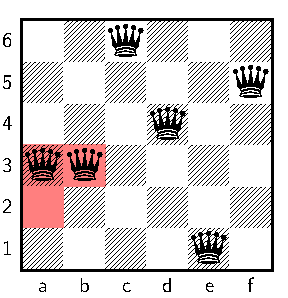
\includegraphics[width=\textwidth]{fig7_scissored.pdf}
  % \chessboard[maxfield=f6, setpieces={qa3,qb3,qc6,qd4,qe1,qf5}]
  \caption{Exemple de position insoluble avec $\eta=0$.}
  \label{fig:echiquier2}
\end{minipage}\qquad%
\begin{minipage}[h]{.55\linewidth}
  \begin{tikzpicture}
    \begin{axis}[%
      width=\textwidth, ymode=log, scaled y ticks=false, scaled x ticks=false,
      xlabel={$n$}, ylabel={Temps de convergence}, legend entries = {Algorithme
        1, Algorithme 2}, legend style = {legend pos=north west}]
      \addplot[color=red, mark = *] coordinates {
        % (4, 2730) (5, 6280) (6, 89530)
        (7, 110190) (8, 372401) (9, 865766) (10, 5005116) (11, 14883900) (12,
        73200000) }; \addplot[color=blue, mark = triangle*] coordinates {
        % (4, 837) (5, 1590) (6,2.78e4)
        (7, 2.49e4) (8, 9.63e4) (9, 1.91e5) (10, 4.74e5) (11, 9.44e5) (12,
        1.78e6) };
      % \addlegendentry{Temps de convergence}
    \end{axis}
  \end{tikzpicture}
  \caption{Temps de convergence moyen selon~$n$.}
  \label{fig:convmoy2}
\end{minipage}
\end{figure}

%\medskip

On veut donc que le choix de la destination ne soit pas toujours la case adjacente qui minimise~$\omega$. On se donne donc une probabilité $\eta \in [0,1]$, et on choisit avec une probabilité $\eta$ une case aléatoire de $V_c$ comme destination, et avec une probabilité $1 - \eta$ une case aléatoire parmi les éléments de~$V_c$ qui minimisent $\omega$. Ainsi, la position de la Figure~\ref{fig:echiquier2} ne pose pas de problème pour $\eta > 0$ : une reine va finir par sortir du triangle rouge et une des autres reines se déplacera par la suite.

Une fois la destination choisie, la procédure qui décide si le déplacement se fait ou non est exactement la fonction $\M$ de l'algorithme précédent.

%\bigskip

% \begin{figure}
%   \centering

%   \begin{minipage}[h]{.45\linewidth}
%     \begin{tikzpicture}
%       \begin{axis}[%
%         width=.55\textwidth, ymode=log, scaled y ticks=false, scaled x
%         ticks=false, xlabel={$n$}, ylabel={Temps de convergence}, legend entries
%         = {Algorithme 1, Algorithme 2}, legend style = {legend pos=north west}]
%         \addplot[color=red, mark = *] coordinates {
%           % (4, 2730) (5, 6280) (6, 89530)
%           (7, 110190) (8, 372401) (9, 865766) (10, 5005116) (11, 14883900) (12,
%           73200000) }; \addplot[color=blue, mark = triangle*] coordinates {
%           % (4, 837) (5, 1590) (6,2.78e4)
%           (7, 2.49e4) (8, 9.63e4) (9, 1.91e5) (10, 4.74e5) (11, 9.44e5) (12,
%           1.78e6) };
%         % \addlegendentry{Temps de convergence}
        
%       \end{axis}
%     \end{tikzpicture}
%     \caption{Temps de convergence moyen en fonction de~$n$.}
%   \end{minipage}\quad%
%   \begin{minipage}[h]{.45\linewidth}
    
%   \end{minipage}
% \end{figure}  

La  Figure~\ref{fig:convmoy2} montre  que  ce nouvel  algorithme  passe mieux  à
l'échelle que  précédemment : la pente de  la courbe qui représente  le temps de
convergence moyen en  fonction de~$n$ est plus faible  pour le nouvel algorithme
que  pour l'ancien.  De  fait, il  permet  de trouver  en  un temps  raisonnable
(quelques minutes  sur une machine  individuelle) des solutions  jusqu'à $n=16$,
contre $12$  pour le modèle précédent, alors  que les temps de  calcul sont très
similaires pour $n=8$. 

% Ceci peut s'expliquer par le fait  que les mouvements sont plus dirigés que dans
% le premier  algorithme, car on utilise  plus d'informations à chaque  coup et on
% s'efforce de choisir des directions intéressantes pour déplacer les reines.


%\clearpage

%\section{Lien avec la factorisation}

\section{Bilan sur le problème des $n$ reines et lien avec la factorisation}

%\ANNOT{$\rightarrow$ système AC mis au point pour résoudre le pb des
%n-reines. Plusieurs points intéressants sur le comportement...
%Hasard est utile (citer Fat13)}

% \begin{floatingfigure}[r]{.5\textwidth}
% %\begin{figure}[htb]
% \centering
% \begin{tabular}{lllllllll|c}
% &&&&&1&0&1&1&$\times$\\
% \hline
% &&&&&1&0&1&1&1\\
% +&&&&0&0&0&0&.&0 \\
% +&&&1&0&1&1&.&.&1\\
% +&&1&0&1&1&.&.&.&1\\
% \hline
% &1&0&0&0&1&1&1&1&\\
% \end{tabular}
% \caption{Multiplication binaire de $11$ ($1011$ en base 2) par $13$ ($1101$, écrit verticalement de bas en haut). Les lignes non-nulles sont bien égales à translation près.}
% \label{fig:facto}
% %\end{figure}
% \end{floatingfigure}

On est parvenu à élaborer un automate cellulaire qui résout le problème des $n$ reines. Les performances, en temps de calcul, sont cependant  bien inférieures à une simple recherche en profondeur, bien que le caractère purement local des interactions entre cellules permette d'envisager de paralléliser cet algorithme de manière efficace. Par ailleurs, l'utilisation du hasard permet de conserver des règles locales relativement simples tout en assurant l'accessibilité des solutions. Enfin, on tire de ce problème des enseignements utiles pour la suite : les con\-train\-tes à propager qui apparaissent dans le problème de la factorisation  peuvent se traduire de manière assez analogue aux signaux transmis par les cellules de ce modèle en utilisant les propriétés de la multiplication binaire.

% En  effet, les  termes de  l'addition binaire  doivent respecter  une contrainte
% globale :  les lignes non-nulles sont toutes  égales (à la translation  due à la
% retenue près)  : si on pose  la multiplication binaire de~$a$  par~$b$, on somme
% des copies  de~$a$, décalées  de~$i$ crans  vers la gauche  pour tout  $i\in I$,
% avec~$I$ tel que $b = \sum_{i\in I}2^i$ (cf. Figure~\ref{fig:facto}) . Ceci peut
% se traduire  de la façon suivante  : une cellule sur  la même ligne  qu'un 1 (la
% ligne est non nulle) et sur la même diagonale qu'un 1 doit contenir elle-même un
% 1.  On peut donc  envisager de  transmettre des  signaux sur  les lignes  et les
% diagonales pour détecter la présence de 1 avec des règles purement locales.
% \\


%%% Local Variables:
%%% mode: latex
%%% fill-column: 80
%%% ispell-dictionary: "francais"
%%% mode: flyspell
%%% TeX-master: "rapportStage"
%%% End:


%%%%%%%%%%%%%%%%%%%%%%%%%%%%%%%%%%%%%%%%%%%%%%%%%%%%%%%%%%%%%%%%%%%%%%%%%%%%%%%%
% FACTORISATION
%%%%%%%%%%%%%%%%%%%%%%%%%%%%%%%%%%%%%%%%%%%%%%%%%%%%%%%%%%%%%%%%%%%%%%%%%%%%%%%%
\part{Problème de la factorisation}
\label{part:facto}

\documentclass[11pt, openany]{article}
\usepackage{pstricks,pstricks-add,pst-math,pst-xkey}
\usepackage[frenchb]{babel}
%\usepackage{slashbox}
\usepackage{graphicx}
\usepackage{amsmath,amssymb,amstext,amsthm}
%\usepackage{comment}
\usepackage[utf8]{inputenc}
\usepackage[OT1]{fontenc}
\usepackage{pgf,tikz}
\usepackage{pgfplots}
\usepackage{floatpag}
\usepgfmodule{shapes}
\usetikzlibrary{arrows,patterns}
\usepackage[ps]{skak}
\usepackage{chessboard}
\usepackage{import}
\newcounter{moncompteur}
\newtheorem{q}[moncompteur]{ \textbf{Question}}{}
\newtheorem{prop}[moncompteur]{ \textbf{Proposition}}{}
\newtheorem{df}[moncompteur]{ \textbf{Définition}}{}
\newtheorem*{df*}{ \textbf{Définition}}{}
\newtheorem{rem}[moncompteur]{ \textbf{Remarque}}{}
\newtheorem{theo}[moncompteur]{ \textbf{Théorème}}{}
\newtheorem{conj}[moncompteur]{ \textbf{Conjecture}}{}
\newtheorem{cor}[moncompteur]{ \textbf{Corollaire}}{}
\newtheorem{lm}[moncompteur]{ \textbf{Lemme}}{}
%\newtheorem{nota}[moncompteur]{ \textbf{Notation}}{}
%\newtheorem{conv}[moncompteur]{ \textbf{Convention}}{}
\newtheorem{exa}[moncompteur]{ \textbf{Exemple}}{}
\newtheorem{ex}[moncompteur]{ \textbf{Exercice}}{}
%\newtheorem{app}[moncompteur]{ \textbf{Application}}{}
%\newtheorem{prog}[moncompteur]{ \textbf{Algorithme}}{}
%\newtheorem{hyp}[moncompteur]{ \textbf{Hypothèse}}{}
\newenvironment{dem}{\noindent\textbf{Preuve}\\}{\flushright$\blacksquare$\\}
\newcommand{\cg }{[\kern-0.15em [}
\newcommand{\cd}{]\kern-0.15em]}
\newcommand{\R}{\mathbb{R}}
\newcommand{\K}{\mathbb{K}}
\newcommand{\N}{\mathbb{N}}
\newcommand{\Z}{\mathbb{Z}}
\newcommand{\C}{\mathbb{C}}
\newcommand{\U}{\mathbb{U}}
\newcommand{\Q}{\mathbb{Q}}
\newcommand{\B}{\mathbb{B}}
\newcommand{\card}{\mathrm{card}}
\newcommand{\norm}[1]{\left\lVert#1\right\rVert}
\pgfplotsset{compat=1.8}
\newcommand{\La}{\mathcal{L}}
\newcommand{\Ne}{\mathcal{N}}
\newcommand{\D}{\mathcal{D}}
\newcommand{\Ss}{\textsc{safestay}}
\newcommand{\Sg}{\textsc{safego}}
\newcommand{\M}{\textsc{move}}
\newcommand{\E}{\mathcal{E}}
\newcommand{\V}{\mathcal V}
\setlength{\parindent}{0pt}
\newcommand{\myrightleftarrows}[1]{\mathrel{\substack{\xrightarrow{#1} \\[-.6ex] \xleftarrow{#1}}}}
\newcommand{\longrightleftarrows}{\myrightleftarrows{\rule{1cm}{0cm}}}

\newcommand\tikzmark[1]{%
  \tikz[overlay,remember picture,baseline] 
  \node[anchor=base](#1){};}

\newcommand\MyLine[3][]{%
  \begin{tikzpicture}[overlay,remember picture]
    \draw[#1] (#2.north west) -- (#3.south east);
  \end{tikzpicture}}


\graphicspath{{.}}


\begin{document}
\floatpagestyle{plain}
\renewcommand{\labelitemi}{$\bullet$}

\title{Multiplication binaire et factorisation}
\date{}
\author{}
\maketitle



\section*{Position du problème}


On cherche un système dynamique discret qui, étant donné un entier non-premier, trouve un de ses diviseurs non-triviaux. On se base sur la multiplication binaire. En effet, on observe qu'une matrice à coefficients dans $\{0,1\}$ peut s'interpréter comme une multiplication binaire si ses lignes non-nulles sont égales entre elles, comme illustré dans la figure $1$. Les colonnes non-nulles sont alors aussi égales entre elles, et les deux facteurs de la multiplication sont alors lisibles, en base $2$, sur les lignes non-nulles pour l'un, et de bas en haut sur les colonnes non-nulles pour l'autre. Si on pose leur multiplication, toujours en base $2$, on retrouve en effet la matrice de départ décalée d'un cran par ligne vers la gauche (cf. Figure~\ref{fig:ExShift}).




\begin{figure}[h]
\centering
\begin{minipage}[]{0.25\linewidth}

\begin{tabular}{cccc}
1&0&1&1\\
0&0&0&0\\
1&0&1&1\\
1&0&1&1\\
\end{tabular}

\end{minipage}
\quad
\begin{minipage}[]{0.4\linewidth}


\begin{tabular}{lllllllll|c}
&&&&&1&0&1&1&$\times$\\
\hline
&&&&&1&0&1&1&1\\
+&&&&0&0&0&0&.&0 \\
+&&&1&0&1&1&.&.&1\\
+&&1&0&1&1&.&.&.&1\\
\hline
&1&0&0&0&1&1&1&1&\\
\end{tabular}
\end{minipage}
\caption{La matrice de gauche s'interprète comme la multiplication de $11$ ($1011$ horizontalement) par $13$ ($1101$ verticalement, de haut en bas).}
\label{fig:ExShift}
\end{figure}

\begin{df*}
Étant donné une matrice $M$ à coefficients dans $\{0,1\}$, on appelle \emph{somme} de $M$ et on note $\sigma (M)$ l'entier obtenu en sommant ses lignes décalées (cf. Figure~\ref{fig:ExSigma}). Si $M$ représente une multiplication, $\sigma(M)$ est par construction le produit. 
\end{df*}


\begin{figure}[]
\centering
\begin{minipage}[]{0.3\linewidth}
$M=$
\begin{tabular}{cccc}
1&1&0&1\\
0&0&1&1\\
1&0&0&1\\
\end{tabular}
\end{minipage}
\quad
\begin{minipage}[]{0.6\linewidth}
$\sigma(M)=$
\begin{tabular}{llllllll}
&&&&1&1&0&1\\
+&&&0&0&1&1&.\\
+&&1&0&0&1&.&.\\
\hline
&&1&1&0&1&1&1\\
\end{tabular}
$=55$
\end{minipage}
\caption{Exemple de calcul de $\sigma$.}
\label{fig:ExSigma}
\end{figure}

L'idée est donc de partir d'une matrice à coefficients dans $\{0,1\}$ dont la somme vaut le nombre qu'on cherche à factoriser, et de lui appliquer des transformations qui préservent la somme comme invariant jusqu'à atteindre une matrice qui représente une multiplication. Ainsi, notre système n'a pas à vérifier que le produit de cette multiplication est l'entier à factoriser, ce qui simplifie considérablement sa conception.

\section*{Un algorithme}

Soit $n$ le nombre de chiffres en base $2$ du nombre composé $N$ dont on cherche un diviseur non-trivial. On se donne une matrice $M$ de taille $ n-1 \times \lceil \frac{n}{2}\rceil$ de somme $N$. Pour tous $a$ et $b$ différents de $1$ et $N$, et tels que $N = ab$, $a$ ou $b$ est de taille inférieure à $\lceil\frac{n}{2}\rceil$ et l'autre est de taille inférieure à $n-1$, on peut donc représenter leur multiplication à l'aide d'une matrice de la taille de $M$. On l'initialise en recopiant les $n-1$ bits de poids faible de $N$ sur la première ligne, et avec un $1$ en position $(2,1)$ et des zéros partout ailleurs (cf. Figure \ref{fig:init}). On vérifie aisément que $\sigma(M)=N$. 


\begin{figure}[h]
\centering

$21 \Rightarrow \overline{10101}^2 \Rightarrow$
\begin{tabular}{cccc}
0&1&0&1\\
1&0&0&0\\
0&0&0&0\\
\end{tabular}
$\Rightarrow$
\begin{tabular}{ccccccc}
&&&0&1&0&1\\
+&&1&0&0&0&.\\
+&0&0&0&0&.&.\\
\hline
&0&1&0&1&0&1\\
\end{tabular}

\caption{Exemple de construction de la matrice $M$ de départ pour factoriser $N=21$.}
\label{fig:init}
\end{figure}

Formellement, on pose $\La=\cg 1, n-1 \cd \times \cg 1, \lceil\frac{n}{2}\rceil\cd$ l'ensemble des cases de la matrice, et $\E=\{0,1\}^\La$ l'ensemble des configurations. Pour tout $x \in \E$, $(i,j)\in\La$, on note $x_{i,j}$ le coefficient $(i,j)$ de la matrice $x$. 

On se donne également un ensemble $\Gamma \subset \E^{\E\times\La}$ de transformations locales qui préservent l'invariant de somme. Elles sont représentées sur la figure~\ref{fig:rules}, et s'appliquent aux coefficients indiqués en gras sous certaines conditions. Les règles \textbf{R5} et \textbf{R6} ne sont en fait pas nécessaires pour l'accessibilité des solutions : on les introduit par symétrie, pour ne pas privilégier de direction de déplacements des $1$. 

%On se donne donc un ensemble $\Gamma$ de six transformations locales qui conservent $\sigma$. Elles sont représentées sur la figure $3$. Plus 


\begin{figure}
\centering
\[
\begin{tabular}{cc}
\textbf 1& \\
 &0\\
\end{tabular}
\mathrel{\mathop{\longrightleftarrows}^{\mathrm{R1}}_{\mathrm{R2}}}
\begin{tabular}{cc}
\textbf 0& \\
 &1\\
\end{tabular}
\]


\[
\begin{tabular}{cc}
0& \\
\textbf 1&0\\
\end{tabular}
\mathrel{\mathop{\longrightleftarrows}^{\mathrm{R3}}_{\mathrm{R4}}}
\begin{tabular}{cc}
1& \\
\textbf 0&1\\
\end{tabular}
\]

\[
\begin{tabular}{ccc}
\textbf 1&0&\\
&&0\\
\end{tabular}
\mathrel{\mathop{\longrightleftarrows}^{\mathrm{R5}}_{\mathrm{R6}}}
\begin{tabular}{ccc}
\textbf 0&1&\\
&&1\\
\end{tabular}
\]

\caption{Transformations locales préservant l'invariant de somme.}
\label{fig:rules}
\end{figure}


%À chaque pas de temps, on choisit au hasard une case et une transformation de $\Gamma$, et on décide si on applique ou non la transformation.


Une formulation équivalente de l'égalité des lignes non-nulles est qu'un coefficient situé sur la même ligne qu'un 1 et sur la même colonne qu'un 1 vaut nécessairement 1 dans une matrice qui représente une multiplication. On va donc appliquer aléatoirement des règles conservant $\sigma$, en privilégiant les mouvements qui retirent les zéros de telles cases. Dans la suite, on dira qu'une case est \emph{sûre} s'il n'y a pas de $1$ sur la même ligne ou s'il n'y en a pas sur la même colonne, et \emph{dangereuse} s'il y a à la fois un $1$ sur la même ligne et un sur la même colonne.

Pour diriger les zéros vers les cases sûres, on voudrait n'effectuer que des mouvements qui sortent un zéro d'une case dangereuse, mais cette restriction est trop forte : il existe alors des situations bloquées, la figure~\ref{fig:stuck} en donne un exemple. Il est donc nécessaire d'autoriser au moins certains mouvements qui ne sont pas directement utiles en ce sens. Par ailleurs, on pourrait vouloir restreindre les mouvements des zéros vers des cases dangereuses, de la même façon que pour le problème des $n$ reines. Cependant, il se forme alors des blocs stables de $1$ : les zéros qui viennent remplacer un $1$ du bord du bloc en sont rapidement éjectés (les seules cases sûres proches sont à l'extérieur du bloc). 

On prend donc le parti de ne pas restreindre les mouvements des zéros vers des cases dangereuses, et on se donne une probabilité d'agitation $p$ : un mouvement valide mais qui ne sort pas un zéro d'une case dangereuse est effectué avec une probabilité $p$, alors qu'un mouvement valide qui sort un zéro d'une case dangereuse est toujours effectué. Dans tous les cas, on ne s'intéresse pas au caractère sûr ou dangereux de la case de destination. 



\begin{figure}
\centering
\begin{tabular}{cccccccc}
0&1&0&0&1&1&0&\fbox 0\\ 
0&\fbox 0&0&0&1&1&0&1\\
0&\fbox 0&0&0&1&1&0&1\\
0&0&0&0&0&0&0&0\\
0&\fbox 0&0&0&1&1&0&1\\
\end{tabular}


\caption{Exemple de situation bloquée si on interdit les mouvements ne déplaçant pas les zéros menacés (encadrés) : aucune des règles de la Figure $3$ ne s'applique à eux.}
\label{fig:stuck}
\end{figure}

À chaque pas de temps, on choisit donc une case de $\La$ et une règle de $\Gamma$ au hasard, et on applique éventuellement la règle à la case. À titre d'exemple, si on choisit, dans une configuration $x$, la case $(i,j)$ et la règle \textbf{R1}, la nouvelle configuration est \[
\textbf{R1}(x,(i,j))=
\begin{cases}
  \hfill x' \hfill & \text{ si}  \begin{cases}\text{ $x_{i,j}=1$ et $x_{i+1,j+1}=0$ }\\
    \text{ et}  \left\{
        \begin{tabular}{@{}c@{}l}
          &\text{ $(i+1,j+1)$ est une case dangereuse}\\
          \text {ou}&\\
          &\text{ $\mathcal{B}(p)=1$}\\
        \end{tabular}
      \right.
  \end{cases}
  \\
  \hfill x \hfill & \text{ sinon}
\end{cases}
\]

avec $x'$ la configuration obtenue à partir de $x$ en échangeant les valeurs de $x_{i,j}$ et $x_{i+1,j+1}$, et $\mathcal{B}(p)$ une variable aléatoire valant $1$ avec une probabilité $p$ et $0$ avec une probabilité $1-p$.

On applique une règle si au moins un des zéros concernés est sur une case dangereuse : ainsi \[
\textbf{R3}(x,(i,j))=
\begin{cases}
  \hfill x'' \hfill & \text {si} \begin{cases}\text{ $x_{i,j}=1$ et $x_{i-1,j}=x_{i,j+1}=0$} \\
    \text{ et} \left\{
        \begin{tabular}{@{}c@{}l}
          &\text{ $(i-1,j)$ est une case dangereuse}\\
          \text {ou}& \text{ $(i,j+1)$ l'est}\\
          \text {ou}& \text{ $\mathcal{B}(p)=1$}\\
        \end{tabular}
      \right.
    \end{cases}
  \\
  \hfill x \hfill & \text {sinon}
\end{cases}
\]

avec $x''$ la configuration obtenue à partir de $x$ en changeant les valeurs de $x_{i,j}$, $x_{i-1,j}$ et $x_{i,j+1}$.

\medskip

Du fait de l'existence de mouvements spontanés, il n'y a pas de point fixe à proprement parler : on est contraint de vérifier après chaque mouvement si la matrice représente une multiplication valide, et d'arrêter les mises à jour le cas échéant. 

\subsection*{Atteignabilité de la solution}

On cherche ici à montrer que la solution est accessible à partir de toute configuration initiale valide en appliquant uniquement les règles de $\Gamma$. On va en fait montrer un résultat un peu plus général : en appliquant les règles de $\Gamma$, il est possible de passer d'une matrice quelconque à n'importe quelle autre matrice de même somme. On suppose fixée la taille des matrices considérées, mais on ne la suppose pas nécessairement égale à celle qu'on utilise dans l'algorithme : cette généralisation permet d'adapter la preuve à des améliorations de l'algorithme.

\begin{df*}
Pour toutes matrices $A$ et $B$, on a $A\sim B$ si et seulement si on peut passer de $A$ à $B$ en appliquant des transformations de $\Gamma$.
\end{df*}

Remarquons que $\sim$ est une relation d'équivalence (la symétrie vient du fait que toutes les règles de $\Gamma$ ont un inverse, donc tous les mouvements sont réversibles).

Pour toute matrice $M$, on numérote ses diagonales descendantes en commençant à $0$ par celle réduite au coin supérieur droit (cf Fig. \ref{fig:diags}), et on note $b_i$ le nombre de coefficients égaux à $1$ sur la diagonale $i$, de sorte que $\sigma (M) = \sum\limits_ib_i2^i$. On constate que deux matrices ayant les mêmes coefficients $b_i$ pour tout $i$ sont équivalentes pour $\sim$ (en fait, on peut passer de l'une à l'autre en utilisant uniquement les règles \textbf{R1} et \textbf{R2}). On note de plus $r$ le nombre de diagonales descendantes de la matrice (si la matrice est de taille $n\times p$, alors $r = n+p+1$). Enfin, pour tout $0\leq i < r$, on note $t_i$ la taille de la $i$-ème diagonale : on a $0\leq b_i \leq t_i$. 
 


\begin{figure}[hbt]
\centering
%\begin{tikzpicture}
%\
%\begin{matrix}
%\tikzmark{a} & \tikzmark{b} & \tikzmark{c} & \\
%\phantom{0}\tikzmark{a21}& & \phantom{0}\tikzmark{a23}& b_0 \\
%\phantom{0}\tikzmark{a31}& \phantom{0}\tikzmark{a32} &  \phantom{0}\tikzmark{a33} & b_1 \\
%&b_4&b_3&b_2\\
%\end{matrix}
%\]
%\end{tikzpicture}

\scalebox{0.3}{\subimport{.}{figdiag.pdf_t}}

\caption{Signification des coefficients $b_i$.}
\label{fig:diags}
\end{figure}

On va montrer que pour tout $N$, toute matrice de somme $N$ est équivalente pour $\sim$ à une certaine matrice qui contient un nombre minimal de $1$.

Soit donc $N \in \N$, $m$ le nombre minimal de $1$ que doit contenir une matrice $M$ de somme $N$. Soit $M$ une telle matrice. Elle vérifie nécessairement, pour tout $i<r-1$, $b_i \leq 1$ ou $b_{i+1}=t_{i+1}$ : sinon, on pourrait appliquer les règles \textbf{R1} et \textbf{R2} dans les diagonales $i$ et $i+1$, puis une fois la règle \textbf{R4} et se ramener à une matrice avec strictement moins de $1$.
Par conséquent, si $b_i > 1$, on a par récurrence que pour tout $j>i$, $b_j = t_j$.
On suppose que tous les coefficients de $M$ ne sont pas égaux à $1$ (sinon, $M$ telle que $\sigma = N$ et on a fini).
Il existe alors $k \in \cg 0, r-1 \cd$ tel que $b_k<t_k$, pour tout  $i<k$, $b_i \leq 1$ et pour tout $i>k$, $b_i=t_i$ ($k$ est le plus grand $i$ tel que $b_i < t_i$).

Soit maintenant $M'$ une autre matrice telle que $\sigma (M')=N$, et minimale pour le nombre de coefficients égaux à $1$ dans sa classe d'équivalence pour~$\sim$. Notons, pour tout $i$, $b'_i$ le nombre de coefficients égaux à $1$ sur la $i$-ème diagonale de $M'$. Il existe également $k'$ tel que $b'_{k'} < t_{k'}$, pour tout $i<k'$, $b'_i \leq 1$ et pour tout $i>k'$, $b'_i=t_i$. Si $k'<k$, alors pour tout $i>k$, $b_i= b'_i$ donc : 

%\begin{align*}
%something\\
%something else
%\end{align*}

\begin{align*}
\sum\limits_{i=0}^{r-1}b_i 2^i = N &= \sum\limits_{i=0}^{r-1}b'_i 2^i\\
\sum\limits_{i=0}^k b_i 2^i &= \sum\limits_{i=0}^k b'_i 2^i\\
b_k 2^k + \underbrace{\sum\limits_{i=0}^{k-1} b_i 2^i}_{\text{$< 2^k$ car $b_i \leq 1$ pour $i<k$}} &=\underbrace{\sum\limits_{i=k'+1}^k t_i 2^i + b_{k'} 2^{k'} + \sum\limits_{i=0}^{k' -1} b_i 2^i}_{\geq t_k 2^k}\\
\end{align*}
ce qui nous amène à une contradiction, car $b_k<t_k$. D'où $k \leq k'$, et par symétrie $k = k'$. Mais alors pour tout $i<k$, $b_i = b'_i$ par unicité de la décomposition en base $2$ du reste de $N$ modulo $2^k$, et pour tout $i>k$, $b_i = b'_i = t_i$, donc on a aussi $b_k = b'_k$ (car $\sum\limits_{i=0}^{r-1} b_i 2^i = \sum\limits_{i=0}^{r-1} b'_i 2^i = N$).

D'où $M' \sim M$. 

Soit donc $A$ telle que $\sigma(A)=N$, et $A'$ la matrice avec le moins de $1$ dans la classe d'équi\-valence de $A$. Clairement $A \sim A'$, or on a vu $A'\sim M$ par minimalité de $A'$ dans sa classe d'équivalence. D'où par transitivité, $A \sim M$. Enfin, toujours par transitivité, si $B$ est une autre matrice de somme $N$, alors $B \sim M$ comme précédemment, donc $A \sim B$.

Toutes les matrices de même somme sont donc équivalentes pour $\sim$, donc on peut passer de l'une à l'autre en appliquant des règles de $\Gamma$. En particulier, toute solution est accessible à partir de toute configuration initiale valide, c'est-à-dire de même somme. 



\section*{Performances et observations}

Les performances varient grandement selon l'entier à factoriser : sa dé\-composition en facteurs premiers, et plus généralement la distribution de $1$ dans la ou les solutions semblent être des facteurs déterminants. Ainsi, les nombres les plus faciles semblent être ceux qui ont le plus de diviseurs, ce qui s'explique par le fait que plus de solutions existent pour de tels nombres. Si on ne s'intéresse qu'aux nombres qui sont le produit de deux nombres premiers, les nombres pour lesquelles les matrices solutions du problème comportent peu de $1$ semblent les plus difficiles : l'algorithme trouve en $10^6$ pas de temps en moyenne un diviseur de $493$ ($ = 17\times 29$), mais pour factoriser $362$ ($ = 2\times 181$), il lui faut $10^9$ étapes ! Ceci est dû au fait que la densité de $1$ varie très peu au cours du temps (elle oscille autour d'une densité moyenne, et les solutions pour lesquelles la densité finale en est éloignée sont difficiles à trouver). 

\medskip

De plus, les conditions que l'on s'est donné pour appliquer les règles tendent à chasser les zéros menacés, mais rien ne pousse particulièrement les $1$ isolés à se déplacer. Il est donc relativement difficile de trouver les positions pour lesquelles les $1$ sont tous à un endroit précis de la matrice : ainsi, pour les nombres de la forme $2^kp$ avec $p$ premier, la matrice aura tous ses $1$ sur la même ligne (la $k$-ième) ou bien sur la même diagonale. Ainsi, dans les cas ``faciles'' tels que $493$, une solution est atteinte environ $40$ fois plus vite avec $p=0.05$ qu'avec $p=1$ (cas où le système applique des règles valides sans tenir compte du caractère dangereux ou sûr des cases), mais dans les cas difficiles tels que $362$, les performances sont plutôt meilleures avec la marche aléatoire $p=1$. Plus généralement, l'évolution du système n'est dirigée que faiblement, notamment parce qu'on a décidé de ne pas restreindre les déplacements de zéros vers des cases dangereuses et parce que le système n'a pas de mémoire.

\medskip
 
Le fait que les $1$ isolés ne soient pas encouragés à se déplacer est d'autant plus gênant qu'on a choisi une taille de matrice nécessairement trop grande pour les facteurs que l'on va trouver. En effet, on a pris une matrice de taille $n-1 \times \lceil \frac{n}{2} \rceil$ pour un nombre de taille $n$ afin d'assurer de pouvoir trouver n'importe quel diviseur non trivial, mais la somme des longueurs des deux facteurs que l'on va trouver est au plus $n+1$. Par conséquent, tous les $1$ d'une matrice solution sont contenus dans un rectangle dont l'un des sommets est le coin supérieur droit et dont le périmètre est limité : s'il y a un $1$ dans le coin inférieur droit, il ne peut y en avoir aucun dans toute la moitié gauche de la matrice ! Si, dans une exécution de l'algorithme, aucun $1$ n'apparaît typiquement dans le quart inférieur gauche pour $p$ assez petit, il y en a fréquemment à la fois dans le coin supérieur gauche et inférieur droit, ce qui fait perdre beaucoup de temps. 


\begin{figure}
  \centering
  \begin{tikzpicture}
  \begin{axis}[%
      width=\textwidth,
      ymode=log,
      scaled y ticks=false,
      %scaled x ticks=false,
      xlabel={$p$},
      ylabel={Temps de convergence},
      xtick = {0.001, 0.01, 0.05, 0.1%, 0.2
      },
      xticklabel style = {
        /pgf/number format/fixed,
       /pgf/number format/precision=3
      },
      legend entries = {221, 247, 319, 377, 403, 493},
      legend style = {legend pos=north west}]
      \addplot coordinates {
        (0.001, 4.3e5) (0.01, 1.6e5) (0.05, 2.4e5) (0.1, 2.4e5) %(0.2, 4.6e5)
      }; 
      \addplot coordinates {
        (0.001, 9.6e4) (0.01, 5.4e4) (0.05, 7.1e4) (0.1, 1.3e5) %(0.2, 1.9e5)
      }; 
      \addplot coordinates {
        (0.001, 9.4e4) (0.01, 5.2e4) (0.05, 8.3e4) (0.1, 1.5e5) %(0.2, 3.0e5)
      }; 
      \addplot coordinates {
        (0.001, 5.7e4) (0.01, 3.9e4) (0.05, 7.7e4) (0.1, 1.6e5) %(0.2, 3.4e5)
      }; 
      \addplot coordinates {
        (0.001, 1.8e5) (0.01, 8.1e4) (0.05, 1.7e5) (0.1, 3.0e5) %(0.2, 8.0e5)
      }; 
      \addplot coordinates {
        (0.001, 5.5e5) (0.01, 5.1e5) (0.05, 8.6e5) (0.1, 1.7e6) %(0.2, 3.6e6)
      }; 

    %\addlegendentry{Temps de convergence}
        
  \end{axis}
  \end{tikzpicture}
  \caption{Temps de convergence moyen en fonction de $N$ et $p$ (échelle logarithmique).}
  \label{fig:p_ag}
\end{figure}  



%TODO : comparatif entre différents entiers


\section*{Quelques améliorations}

\subsection*{Fixer la taille des diviseurs recherchés}

On peut donc envisager l'amélioration suivante : plutôt que d'utiliser une grande matrice, on suppose connue la taille des diviseurs. Si $n$ est la taille du nombre à factoriser, il y a au plus $2n-1$ tailles de matrices possibles à essayer car la somme des tailles des diviseurs vaut nécessairement $n$ ou $n+1$ et on ignore les matrices dont une dimension vaut $1$ car on cherche des diviseurs non-triviaux. On lance donc en parallèle l'algorithme sur les $2n-1$ matrices différentes, et on arrête l'exécution dès qu'une solution est trouvée pour l'une des tailles. Quitte à supposer impair le nombre à factoriser, on impose de plus qu'il y ait un $1$ à chacun des quatre coins (c'est une condition nécessaire pour qu'une matrice dont les dimensions sont exactement les tailles de deux facteurs soit solution : chaque facteur commence par un $1$ car les zéros à gauche ne sont pas significatifs, et finissent par un $1$ car les diviseurs d'un nombre impair sont impairs). 

\medskip
Il apparaît que l'exécution de l'algorithme est significativement plus rapide qu'avec la grande matrice. Les nombres dont l'un des facteurs est très petit deviennent très faciles à traiter, car la matrice de la bonne taille est très petite, et le calcul y aboutit donc rapidement. Les nombres les plus difficiles à traiter deviennent, comme pour les algorithmes classiques de factorisation, les produits de deux nombres premiers de même taille : en effet, la seule matrice pour laquelle l'algorithme peut aboutir est alors de taille maximale. Même dans ce cas, l'exécution est plus rapide car on ne perd plus de temps à cause des $1$ situés dans une zone inutile de la matrice. On gagne ainsi un facteur $100$ sur le temps de factorisation de $329$ ($ =7\times 47$), largement de quoi justifier le lancement simultané d'une quinzaine d'exécutions. % TODO : stats plus détaillées ici ?

%TODO : comparatif entre différents entiers
%TODO : comparatif entre fact0 et fact_fixed_lengths

\subsection*{Permettre des échanges à plus longue distance}

Les transformations préservant l'invariant de somme introduites plus haut sont très localisées : on peut envisager de remplacer les règles \textbf{R1} et \textbf{R2} par une règle plus générale, qui consiste à intervertir deux cellules situées sur la même diagonale descendante. De même, on peut remplacer les règles \textbf{R3} et \textbf{R5} par une règle qui consiste à échanger un $1$ d'une diagonale contre deux sur la diagonale à sa droite, et les règles \textbf{R4} et \textbf{R6} par une règle qui consiste à échanger un $0$ d'une diagonale contre deux sur la diagonale à sa droite. Les transformations du système sont ainsi plus équitables au sens où on peut maintenant atteindre, en appliquant une seule règle, des positions qu'on ne pouvait précédemment atteindre que par une séquence précise de transformations locales. 

Il semble cependant que ce changement n'améliore pas significativement le temps mis pour atteindre une solution : pour certains entiers à factoriser, on constate une amélioration de l'ordre de $10\%$, mais pour d'autres, le temps de convergence subit au contraire une augmentation du même ordre.   

%TODO : comparatif entre fact_fixed_lengths et fact_global

\subsection*{N'utiliser que des informations locales}

Dans l'algorithme ci-dessus, on utilise des informations globales sur le système lorsqu'on décide si on applique une transformation : en effet, on décide si une case est sûre ou dangereuse en comptant les $1$ sur la ligne et la diagonale concernées. On peut en fait ajuster l'algorithme pour se restreindre à utiliser uniquement des informations locales, en mettant en place un système de signaux analogue à celui utilisé pour le problème des $n$ reines. 

On procède de la façon suivante : les cellules de la matrice, en plus de contenir un $0$ ou un $1$, peuvent contenir des signaux en provenance des quatre directions $N$, $S$, $E$ et $W$. On souhaite qu'un signal en provenance d'une certaine direction soit présent sur une cellule s'il existe un coefficient égal à $1$ dans cette direction. Ainsi, une case est dite \emph{sûre} si elle ne contient pas de signal en provenance du nord ni du sud, ou bien si elle ne contient pas de signal en provenance de l'ouest ni de l'est. Dans le cas contraire, elle est dite \emph{dangereuse}. On a ainsi traduit l'ancienne définition d'une cellule sûre (pas de $1$ sur la même colonne, ou bien pas de $1$ sur la même ligne) en terme de signaux.

À chaque pas de temps, on choisit une cellule $c$ à mettre à jour et on commence par mettre à jour ses signaux de la même façon que pour le problème des $n$ reines : pour chaque direction $d$, si $c'$ est la cellule voisine de $c$ dans la direction $d$, le signal en $c$ en provenance de la direction $d$ devient présent si $c'$ contient un $1$, et prend le même état (présent ou absent) que celui de $c'$ en direction de $d$ sinon.
Après avoir mis les signaux de $c$ à jour, on applique l'algorithme précédent pour décider si on applique une transformation de $\Gamma$, en utilisant la nouvelle définition de case sûre/dangereuse. 

Comme on pouvait s'y attendre, on constate une déterioration des performances lorsqu'on se restreint ainsi à des informations locales. Cependant, cette augmentation du temps mis à atteindre une solution reste raisonnable, ce qui est prometteur dans le sens où se restreindre à des informations locales peut permettre de paralléliser le système en effectuant plusieurs mises à jour simultanées, sans conflits à condition que les zones affectées par les différentes mises à jour soient disjointes. Ceci était moins efficace avec l'algorithme initial du fait de la nécessité de garder une trace du nombre total de $1$ sur chaque ligne et diagonale, ce qui impose de centraliser les mises à jour sous peine d'en effectuer certaines avec des informations erronées.

%TODO : comparatif entre fact_fixed_lengths et fact_sigs

\nocite{Pom96}
\nocite{BahiC06}
\nocite{Fat13}

\bibliographystyle{plain}
\bibliography{bibfact}

\end{document}



%%%%%%%%%%%%%%%%%%%%%%%%%%%%%%%%%%%%%%%%%%%%%%%%%%%%%%%%%%%%%%%%%%%%%%%%%%%%%%%%
% CONCLUSION
%%%%%%%%%%%%%%%%%%%%%%%%%%%%%%%%%%%%%%%%%%%%%%%%%%%%%%%%%%%%%%%%%%%%%%%%%%%%%%%%


\part*{Conclusion}

...


\bibliographystyle{plain}
\bibliography{biblio}

\end{document}

%%% Local Variables:
%%% mode: latex
%%% fill-column: 80
%%% ispell-dictionary: "francais"
%%% mode: flyspell
%%% TeX-master: t
%%% End:
